% -----------------
%  UNIVERSITY OF LIMERICK

% Based on Giuseppe Torre 2020 template, here is a version Gauri Vaidya has modified.

% ------------------


%: Style file for Latex
% Most style definitions are in the external file PhDthesisPSnPDF.
% In this template package, it can be found in ./Latex/Classes/
\documentclass[twoside,12pt]{Latex/Classes/PhDthesisPSnPDF}
\newcommand{\frontmatter}{
  \cleardoublepage
  \pagenumbering{roman}
  \setcounter{page}{1}
}
\usepackage{lmodern}
\usepackage{graphicx}
\usepackage{subscript}
% \usepackage{textcomp}
\usepackage{newtxmath}
\DeclareUnicodeCharacter{03BC}{\textmu}
\makeatletter
\@ifundefined{ver@xcolor.sty}{\RequirePackage{xcolor}}{}
\makeatother
\newcommand{\conor}[1]{\textcolor{red}{\textbf{\textit{#1}}}}
\newcommand{\meghana}[1]{\textcolor{blue}{\textbf{\textit{#1}}}}
\newcommand{\gauri}[1]{\textcolor{orange}{\textbf{\textit{#1}}}}
\usepackage{natbib}
\usepackage{url}
\usepackage[utf8]{inputenc}
\usepackage{textcomp}
\usepackage{amssymb}
\usepackage{amsfonts}
\usepackage{textgreek}
\usepackage{url}
\usepackage[utf8]{inputenc}
\usepackage{alltt} 
\usepackage{multirow}
\usepackage{color}
\usepackage{boldline}
\usepackage{arydshln}
\usepackage{algorithmicx}
\usepackage{algorithm}
\usepackage{algpseudocode}
\usepackage{algforeach}
\usepackage{amsmath}
\usepackage{caption}
\usepackage{subcaption}
\usepackage{booktabs}
\usepackage{array}
\usepackage{paralist}  
\usepackage{enumitem}  
\usepackage{adjustbox}
\usepackage{newtxtext}

% to display Math
\usepackage{mathtools}
% to Display C++ code
\definecolor{c++red}{rgb}{0.6,0,0} % for strings
\definecolor{c++green}{rgb}{0.25,0.5,0.35} % comments
\definecolor{c++purple}{rgb}{0.5,0,0.35} % keyword
\usepackage{listings}
\lstset{language=C++}

\newcommand{\webfootnote}[2]{\footnote{\url{#1} \textit{Retrieved #2}}}

\makeatletter  
\def\url@leostyle{%
  \@ifundefined{selectfont}{\def\UrlFont{\sf}}{\def\UrlFont{\small\ttfamily}}}
\makeatother
%% Now actually use the newly defined style.
\urlstyle{leo}

%: Macro file for Latex
% Macros help you summarise frequently repeated Latex commands.
% Here, they are placed in an external file /Latex/Macros/MacroFile1.tex
% An macro that you may use frequently is the figuremacro (see introduction.tex)



%: ----------------------------------------------------------------------
%:                  TITLE PAGE: name, degree,..t
% ----------------------------------------------------------------------
% below is to generate the title page with crest and author name

%if output to PDF then put the following in PDF header
\ifpdf  
    \pdfinfo { /Title  (PhD and MPhil Thesis Classes)
               /Creator (TeX)
               /Producer (pdfTeX)
               /Author (Name email address)
               /CreationDate (20241206)  %format D:YYYYMMDDhhmmss
               /ModDate (D:YYYYMMDDhhmm)
               /Subject (Main subjects of your thesis)
               /Keywords (put here few keywords relevant to your PhD work) }
    \pdfcatalog { /PageMode (/UseOutlines)
                  /OpenAction (fitbh)  }
\fi


\title{Title}



% ----------------------------------------------------------------------
% The section below defines www links/email for author and institutions
% They will appear on the title page of the PDF and can be clicked
\ifpdf
  \author{\href{mailto:}{FirstName LastName}}

% here the links to the Institution you belong to
  \researchcentre{\href{}{Research Group}}
  \faculty{\href{https://www.ul.ie}{Faculty}}
  \department{\href{https://www.ul.ie}{Department Name}}
  \university{\href{https://www.ul.ie}{University of Limerick}}

  % The crest is a graphics file of the logo of your research institution.
  % Place it in ./0_frontmatter/figures and specify the width
  \crest{
\includegraphics[scale=0.45]{logonew2020.jpg}}


%\renewcommand{\submittedtext}{change the default text here if needed}
\degree{MSc in Artificial Intelligence and Machine Learning}
\degreedate{\today}


% ----------------------------------------------------------------------
       
% turn of those nasty overfull and underfull hboxes
\hbadness=10000
\hfuzz=50pt


%: --------------------------------------------------------------
%:                  FRONT MATTER: dedications, abstract,..
% --------------------------------------------------------------
\usepackage{textalpha}
\begin{document}
\include{Latex/Macros/MacroFile1}

%\language{english}



% sets line spacing
\renewcommand\baselinestretch{1.2}
\baselineskip=16pt plus1pt


%: ----------------------- generate cover page ------------------------

\maketitle  % command to print the title page with above variables


%: ----------------------- cover page back side ------------------------
% Your research institution may require reviewer names, etc.
% This cover back side is required by Dresden Med Fac; uncomment if needed.

\newpage


 \begin{tabbing}
1.  Supervisor: \= Name    \\
 \>  \= Dept Name \\
 \>  \= University \emph{of} Limerick \\
 \>  \= Ireland \\
 \end{tabbing}


 \begin{tabbing}
2. Supervisor: \= Name \\
 \>  \= Dept Name \\
 \>  \= University \emph{of} Limerick \\
 \>  \= Ireland \\
\end{tabbing}

\vspace{10mm}


%: ----------------------- abstract ------------------------

% Your institution may have specific regulations if you need an abstract and where it is to be placed in the document. The default here is just after title.
%: Declaration of originality

\begin{abstracts}  


    The increasing deployment of wind turbines necessitates robust condition monitoring systems to ensure operational reliability and reduce maintenance costs.
    This thesis presents a comprehensive investigation into the capacity of Deep Reconstructive Normal Behaviour Models for anomaly detection in wind turbine SCADA data.
    Moving beyond controlled lab settings, this research leverages a proprietary, realistically labeled industrial dataset to evaluate model performance under conditions that mirror real-world challenges, including class imbalance and previously unseen operational anomalies.

    A systematic comparison of \gls{ae} architectures—including Vanilla, Multi-Head, Classification-Only, and a novel Bottleneck AE — was conducted under unsupervised, semi-supervised, and fully supervised training paradigms.
    Furthermore, an \gls{arae} was proposed to enhance robustness in data-scarce scenarios.
    The impact of auxiliary loss functions (MMD, Wasserstein, Fourier, Mahalanobis) and advanced architectural components (Multi-Scale Attention Memory) was also rigorously evaluated.

    Key experimental results demonstrate that purely unsupervised Vanilla AEs fail to achieve linear separability (AUC $\approx$ 0.5), challenging a common assumption in the literature.
    Performance significantly improved with the introduction of supervisory signals; the Multi-Head AE achieved an AUC of 0.9288 via its classification head and 0.9758 using a classifier on its reconstruction errors.
    The Bottleneck AE, which jointly optimizes reconstruction and classification, achieved near-perfect performance (AUC: 0.9983, F1-score $>$ 99\%).
    For scenarios with limited abnormal data, the proposed ARAE maintained stable recall (0.8547) even at a 1:4 abnormal-to-normal ratio, outperforming other models under severe class imbalance.
    The study also found that distribution-alignment losses (Wasserstein, MMD) effectively complemented MSE, while complex architectural additions often degraded the performance of well-tuned baselines.

    The findings underscore that the success of deep reconstructive models is heavily dependent on architectural choices, the availability of labels, and training strategies.
    This work provides a foundational comparison and a set of validated design patterns, concluding that the Bottleneck AE is optimal when labeled data is abundant, while the ARAE offers a robust and practical path forward for the more common industrial scenario of limited fault examples.

\end{abstracts}


% Thesis statement of originality -------------------------------------

% Depending on the regulations of your faculty you may need a declaration like the one below. This specific one is from the medical faculty of the university of Dresden.

\begin{declaration}       

I herewith declare that I have produced this thesis without the prohibited assistance of third parties and without making use of aids other than those specified; notions taken over directly or indirectly from other sources have been identified as such. This paper has not previously been presented in identical or similar form to any other Irish or foreign examination board.

The thesis work was conducted from 2021 to 2025 under the supervision of \textit{Name of your Supervisor(s)} at University of Limerick.

\vspace{10mm}

Limerick, 2025

\end{declaration}


% ----------------------------------------------------------------------

% Thesis statement of use of Gen AI.

\begin{useofgenai}       

I herewith declare that I have used Gen AI to....

\vspace{10mm}

Limerick, 2025

\end{useofgenai}


% ----------------------------------------------------------------------

%: ----------------------- tie in front matter ------------------------

\frontmatter


\begin{acknowledgements}    

    I would first like to express my sincere gratitude to my direct supervisor, Juan Albarracin. I am deeply thankful for his unwavering responsiveness in answering my questions and addressing my concerns. His willingness to provide meticulous proof-reading and essential knowledge support was fundamental to the progress of this work.

    My special thanks go to Conor Ryan, Head Director of the BDS research group. His remarkable skills and charismatic leadership were truly inspiring and were instrumental in fostering my passion for academic research.

    I am also indebted to the entire BDS group, a community of bright and talented individuals. Though our direct interactions may have been limited, their collective intellect and enthusiasm have been a significant source of influence and encouragement, solidifying my commitment to pursuing a path in artificial intelligence.






\end{acknowledgements}

% ------------------------------------------------------------------------

% Thesis Dedictation ---------------------------------------------------

\begin{dedication} %this creates the heading for the dedication page

\vspace{31mm}

Dedicated to \textit{xyz};

\end{dedication}

% ----------------------------------------------------------------------

%: ----------------------- contents ------------------------

\setcounter{secnumdepth}{3}
\setcounter{tocdepth}{3}
\tableofcontents

\listoftables
\listoffigures
\clearpage


\mainmatter  

\renewcommand{\chaptername}{}  % Optional: suppress "Chapter" label

%: ----------------------- subdocuments ------------------------
% this file is called up by thesis.tex
% content in this file will be fed into the main document

%: ----------------------- introduction file header -----------------------
\chapter{Introduction}

% the code below specifies where the figures are stored
\ifpdf
    \graphicspath{{1_introduction/figures/PNG/}{1_introduction/figures/PDF/}{1_introduction/figures/}}
\else
    \graphicspath{{1_introduction/figures/EPS/}{1_introduction/figures/}}
\fi

This is how you cite~\citep{Moore99}.

Single sample image. 
\begin{figure}[!htbp]
\centering
\centering
   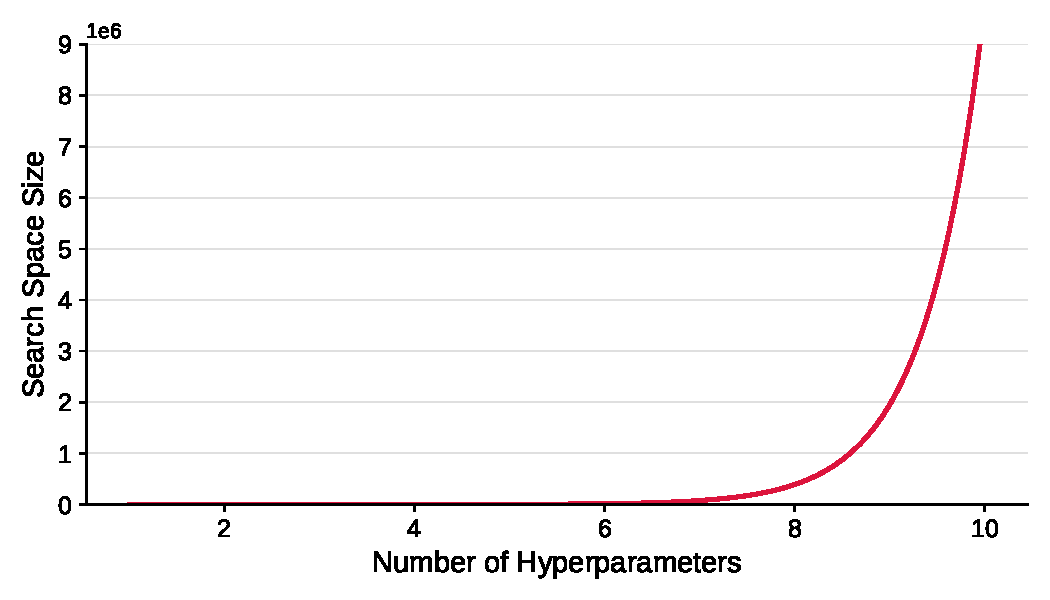
\includegraphics[width=0.8\textwidth]{1_introduction/figures/search_space.pdf}
   \caption{}
   \label{fig:abc}
\end{figure}


Sample subfigures.
\begin{figure}[!htbp]
\centering
\begin{subfigure}[b]{\textwidth}
\centering
   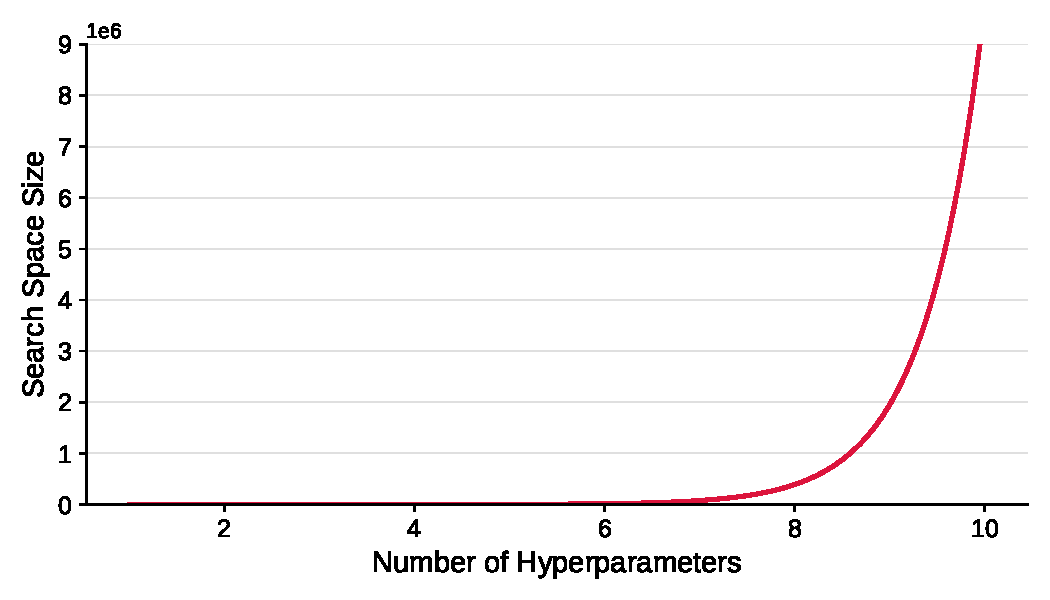
\includegraphics[width=0.4\textwidth]{1_introduction/figures/search_space.pdf}
   \caption{}
   \label{fig:search_space_exp}
\end{subfigure}
\begin{subfigure}[b]{\textwidth}
\centering
   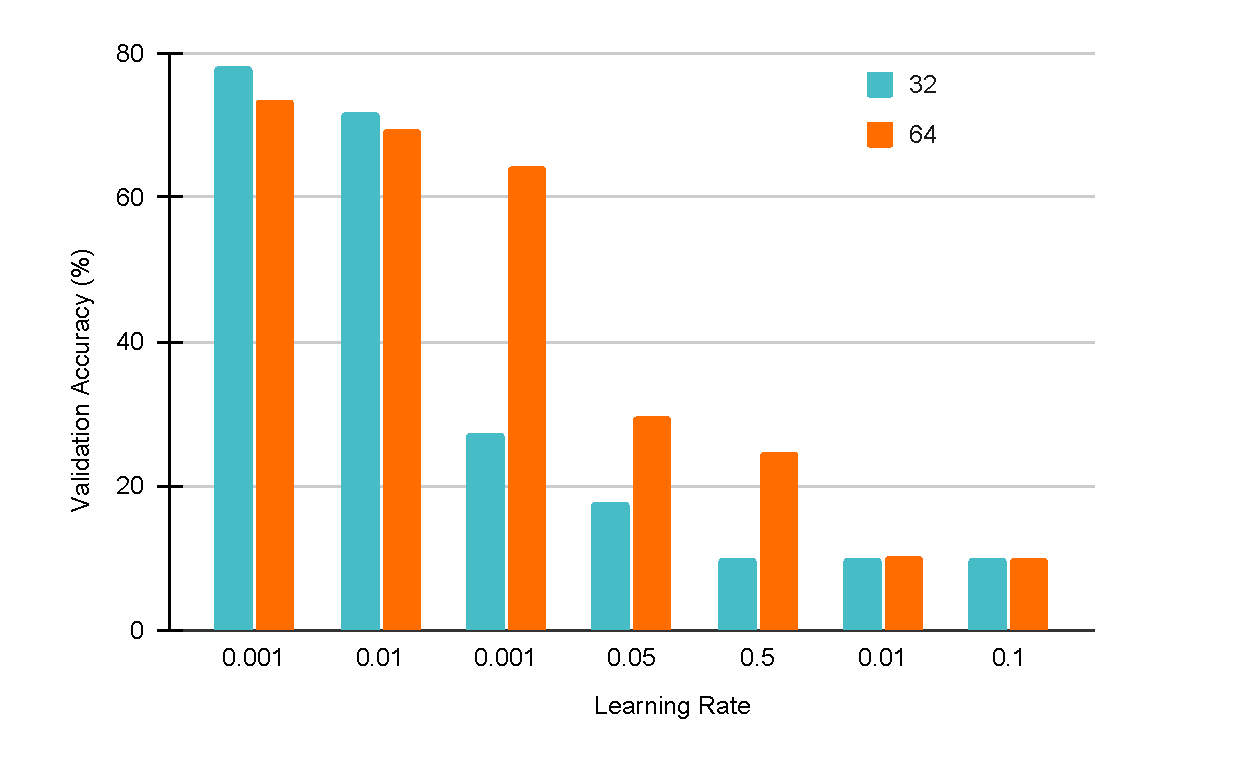
\includegraphics[width=0.4\textwidth]{1_introduction/figures/impact-of-hyp.pdf}
   \caption{}
   \label{fig:impact_hyper}
\end{subfigure}
\begin{subfigure}[c]{\textwidth}
\centering
   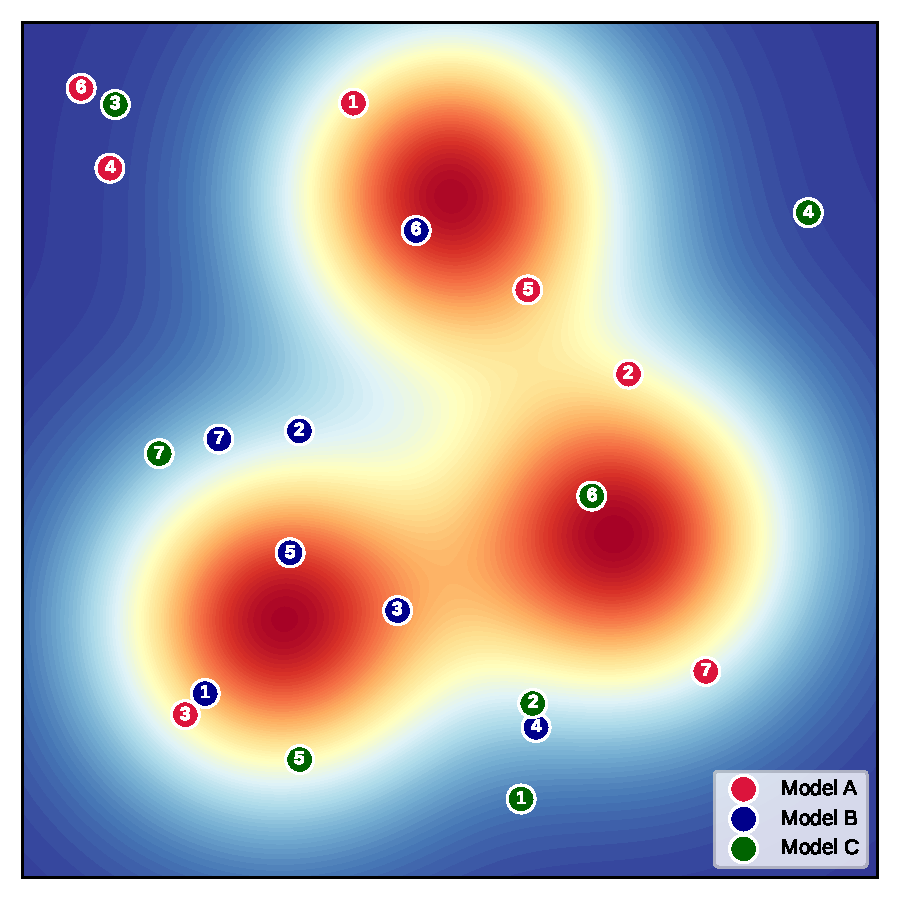
\includegraphics[width=0.4\textwidth]{1_introduction/figures/fitness_landscape.pdf}
   \caption{}
   \label{fig:fitness_landscape}
\end{subfigure}
\caption{Sample.
(a) Caption 1;
(b) Caption 2;
(c) Caption 3.}
\label{fig:challenges}
\end{figure}



% ------------------- Table Start -------------------
\begin{table}[!htb]
\caption{Sample hyperparameter configurations.}
\center
\begin{tabular}{lccc}
\hlineB{2}
\textbf{Optimizer} & \textbf{Learning Rate} & \textbf{Batch Size} & \textbf{Validation Accuracy} \\ \hlineB{2}
adam & \(1.00 \times 10^{-3}\) & 128 & 0.14 \\
adam & \(1.00 \times 10^{-4}\) & 128 & 0.57 \\
rmsprop & \(1.00 \times 10^{-4}\) & 32 & 0.52 \\
rmsprop & \(1.00 \times 10^{-3}\) & 16 & 0.14 \\
rmsprop & \(1.00 \times 10^{-6}\) & 8 & 0.43 \\ \hlineB{2}
\end{tabular}
\label{tab:sample_individuals}
\end{table}
% ------------------- Table End -------------------


% this file is called up by thesis.tex
% content in this file will be fed into the main document

%: ----------------------- introduction file header -----------------------
\chapter{Background}
\label{ch:background}

% the code below specifies where the figures are stored
\ifpdf
    \graphicspath{{2_background/figures/PNG/}{2_background/figures/PDF/}{2_background/figures/}}
\else
    \graphicspath{{2_background/figures/EPS/}{2_background/figures/}}
\fi


\section{Wind Turbine Condition Monitoring}
\label{sec:wt-condition-monitoring}

Wind Turbine Condition Monitoring (WTCM) is the systematic process of continuously or periodically assessing the operational health of wind turbine components, such as gearboxes, bearings, blades, and generators, through the measurement and analysis of operational parameters including vibration, temperature, acoustic emissions, and power output~\citep{li_comprehensive_2023,charabi_wind_2020,henrique_global_nodate}.
The principal objective of WTCM is the early detection of anomalies or degradation, thereby enabling timely maintenance interventions that mitigate the risk of catastrophic failure, minimise unplanned downtime, and sustain optimal energy production throughout the turbine’s service life.

Modern WTCM typically integrates dedicated Condition Monitoring Systems (CMS) with Supervisory Control and Data Acquisition (SCADA) platforms.
CMS record high-frequency sensor data related to mechanical and structural health, whereas SCADA provides low-frequency operational and environmental data, along with historical event logs including failures, repairs, and downtimes~\citep{dao_wind_2019}.
The combined datasets underpin reliability analyses, facilitate the optimisation of operational strategies, and form the foundation for data-driven maintenance planning.

Maintenance activities within the wind energy sector are generally classified into three principal categories~\citep{yang_operations_2021,henrique_global_nodate}:

Reactive (Corrective) Maintenance (CM): Interventions performed only after a failure has occurred or performance has dropped below acceptable thresholds.
While such actions restore operational capability, they are typically associated with elevated costs due to unplanned downtime, emergency repairs, and potential collateral damage to adjacent components.

Condition-Based Maintenance (CBM): A proactive strategy in which maintenance is triggered when monitored parameters, such as vibration or temperature, deviate from predefined operational thresholds.
CBM enables faults to be addressed in their early stages, reducing the likelihood of unplanned outages and extending component lifespan.

Predictive Maintenance (PdM): An advanced form of proactive maintenance that leverages statistical modeling, historical trends, and increasingly, machine learning algorithms to forecast the remaining useful life of components.
Maintenance is scheduled in advance of predicted failures, often incorporating CBM data but focusing on forecasting rather than detection.

The fundamental distinction between these strategies lies in their temporal relationship to component degradation: CBM is driven by current health indicators, PdM anticipates future failure events, and reactive maintenance responds after failures have occurred.
In practice, hybrid maintenance policies are often adopted, combining elements of each strategy to optimise cost, reliability, and risk.
Such hybrid approaches are particularly relevant in offshore wind energy applications, where logistical constraints, weather-related access limitations, and high operational costs necessitate highly efficient maintenance planning~\citep{yang_operations_2021}.


\section{Normal Behaviour Monitoring}
\label{sec:normal-behaviour-monitoring}
Normal Behaviour Monitoring (NBM) refers to the modeling of a system's nominal operational patterns in order to detect deviations that may indicate emerging faults or performance degradation.
In the context of wind turbine condition monitoring, NBM leverages historical and real-time operational data to establish a representation of “healthy” turbine behaviour.
Any statistically significant departure from this model is treated as a potential anomaly warranting further investigation or maintenance intervention.

NBM is particularly relevant for wind turbines due to their complex, non-linear dynamics and the wide variability of environmental conditions under which they operate.
Unlike threshold-based monitoring—where fixed limits on operational parameters trigger alerts—NBM captures multivariate and temporal correlations between signals, providing a more nuanced picture of system health.
However, the accuracy of NBM hinges on the availability of sufficient high-quality “normal” data and the ability of the modeling technique to cope with non-stationary operating regimes (e.g., seasonal wind patterns, load variations).

Modern Supervisory Control and Data Acquisition (SCADA) systems now generate high-frequency time-series telemetry data from various turbine components, enabling what is commonly referred to as NBM—the task of modeling normal operational patterns to detect abnormal deviations.

The methods employed in NBM broadly fall into three categories: statistical approaches, traditional (shallow) machine learning, and deep learning-based methods.

Statistical methods, such as Ordinary Least Squares (OLS), ARIMA, and Principal Component Analysis (PCA), are still used in certain settings~\citep{chesterman_overview_2023}.
These models are computationally efficient, interpretable, and data-efficient, making them suitable for constrained environments or first-pass screening.
However, their simplicity limits their ability to model complex, non-linear system behaviour.

Traditional machine learning models, including Random Forests, Gradient Boosting Machines, and Support Vector Machines, have grown more popular due to their improved performance on non-linear tasks and moderate data requirements.
These methods still require feature engineering and are sensitive to class imbalance, but they offer a strong middle ground in the performance–complexity trade-off~\citep{ben_ali_online_2018, bilendo_normal_2022, liu_wind_2022}.

Deep learning methods—especially neural network-based architectures—have rapidly become the dominant approach in recent research.
These models offer superior capability to capture non-linear dependencies in high-dimensional data but come at the cost of increased computational demand and reduced interpretability.
Within this category, Autoencoders (AEs) have emerged as a popular choice for anomaly detection, particularly in unsupervised or semi-supervised settings.
Like PCA, Autoencoders learn latent representations of normal behaviour via dimensionality reduction, but with significantly greater expressive power due to their ability to model non-linearities.

Accordingly, a growing body of research has focused on applying machine learning (ML) and deep learning (DL) techniques to enable condition monitoring and early fault detection in wind turbines.
Among these, Autoencoders have become one of the most widely adopted architectures for unsupervised and semi-supervised anomaly detection~\citep{chesterman_overview_2023}.

Recent trends point towards deep reconstructive normal behaviour models—architectures that not only learn a latent representation of healthy behaviour but also attempt to reconstruct the original signal.
By analysing reconstruction errors, these models can highlight subtle deviations that may be indicative of incipient faults.
Section~\ref{sec:deep-reconstructive} explores these models in detail, including their theoretical underpinnings, design considerations, and application to wind turbine condition monitoring.

------------------------------------

Modern Supervisory Control and Data Acquisition (SCADA) systems now generate high-frequency time-series telemetry data from various turbine components, enabling what is commonly referred to as Normal Behavior Monitoring (NBM) — the task of modeling normal operational patterns to detect abnormal deviations.

The methods employed in NBM broadly fall into three categories: statistical approaches, traditional (shallow) machine learning, and deep learning-based methods.

Statistical methods, such as Ordinary Least Squares (OLS), ARIMA, and Principal Component Analysis (PCA), are still used in certain settings~\citep{chesterman_overview_2023}.
These models are computationally efficient, interpretable, and data-efficient, making them suitable for constrained environments or first-pass screening.
However, their simplicity makes them less capable of modeling complex, non-linear system behavior.

Traditional machine learning models, including Random Forests, Gradient Boosting Machines, and Support Vector Machines, have grown more popular due to their better performance on non-linear tasks and moderate data requirements.
These methods still require some feature engineering and are sensitive to class imbalance, but they offer a strong middle ground in performance versus complexity trade-offs.
The methods are presented by~\cite{ben_ali_online_2018, bilendo_normal_2022, liu_wind_2022}.

Deep learning methods—especially neural network-based architectures—have rapidly become the dominant approach in recent research.
These models offer superior ability to capture non-linear dependencies in high-dimensional data but come at the cost of increased computational demand and reduced interpretability.
Within this category, Autoencoders (AEs) have emerged as a popular choice for anomaly detection, particularly in unsupervised or semi-supervised settings.
Just like PCA, Autoencoders learn latent representations of normal behavior via dimension reduction, but with significantly more expressive power due to their ability to model non-linearities.

Accordingly, a growing body of research has focused on applying machine learning (ML) and deep learning (DL) techniques to enable condition monitoring and early fault detection in wind turbines.
Among these, Autoencoders (AEs) have emerged as one of the most widely adopted architectures, particularly in unsupervised or semi-supervised anomaly detection settings~\citep{chesterman_overview_2023}.
 
% this file is called up by thesis.tex
% content in this file will be fed into the main document

%: ----------------------- introduction file header -----------------------
\chapter{Related Works}
\label{ch:related-works}

% the code below specifies where the figures are stored
\ifpdf
    \graphicspath{{2_related_works/figures/PNG/}{2_related_works/figures/PDF/}{2_related_works/figures/}}
\else
    \graphicspath{{2_related_works/figures/EPS/}{2_related_works/figures/}}
\fi


\section{Wind Turbine Condition Monitoring}
\label{sec:wind-turbine-condition-monitoring}
\gls{wtcm} plays a central role in reducing operational costs and improving the reliability of both onshore and offshore wind farms.
As Dao et al.
(2019) note, operational and maintenance costs account for approximately 20-30\% of the Levelised Cost of Energy, making early fault detection a key strategy for cost control.
Condition monitoring enables operators to identify incipient failures, minimize unplanned downtime, and optimize energy production through targeted maintenance.
\cite{yang_operations_2021} similarly emphasize that proactive monitoring improves asset longevity and reduces corrective maintenance needs, with particular benefits for offshore installations where accessibility is constrained.

Effective \gls{wtcm} integrates multiple data sources, including \gls{scada} systems, \gls{cms}, and historical failure logs.
\gls{scada} data—capturing variables such as power output, rotor speed, vibration, and temperature—facilitates real-time anomaly detection, while \gls{cms} focuses on mechanical components such as gearboxes, bearings, and drive shafts.
The combination of these sources supports not only short-term operational decisions but also long-term reliability modelling.


\subsection{Traditional Statistical Approaches}
\label{subsec:traditional-statistical-approaches}
Early approaches to \gls{wtcm} relied heavily on statistical models for anomaly detection and degradation trend analysis.
ARIMA models were applied to capture temporal dependencies in \gls{scada} data, particularly for forecasting power output or component temperatures under normal operating conditions~\cite{chesterman_overview_2023}.
\gls{pca} was used to reduce the dimensionality of multivariate datasets and to extract latent features associated with turbine health status.
In parallel, threshold-based monitoring systems compared sensor readings against predefined limits, triggering alarms when deviations exceeded acceptable ranges.

While these statistical methods provided valuable insights in the early stages of \gls{wtcm}, they suffer from notable limitations.
Many approaches assume linear relationships between variables, which rarely hold in the complex, nonlinear dynamics of turbine operation.
Moreover, their scalability to modern high-frequency, high-dimensional \gls{scada} datasets is limited—particularly as offshore wind farms generate terabytes of heterogeneous sensor data.
Threshold-based approaches, in particular, are prone to false alarms when environmental variability (e.g., wind speed fluctuations) is not adequately modelled.



\subsection{Transition to Machine Learning Techniques}
\label{subsec:transition-to-machine-learning-techniques}
The statistical foundations of \gls{wtcm} have directly informed the transition to \gls{ml}-based approaches.

For example, \gls{pca}'s dimensionality reduction principles underpin the structure of autoencoders used for unsupervised anomaly detection.
Similarly, ARIMA's time series modelling concepts inspire \glspl{rnn} and temporal convolutional networks that capture complex, nonlinear dependencies.
Threshold-based methods have evolved into supervised learning classifiers that learn optimal decision boundaries from historical fault data, rather than relying on fixed limits.
As turbine datasets have grown in size and complexity, these \gls{ml} approaches have demonstrated improved fault detection accuracy, adaptability to nonstationary conditions, and robustness to noisy inputs — making them a natural evolution of earlier statistical techniques.


\subsection{Conclusion}
Statistical methods laid the foundation for modern \gls{wtcm} by providing initial frameworks for anomaly detection and fault diagnosis.
However, their inherent limitations in handling non-linearity and high-dimensional data have necessitated the shift toward \textbf{data-driven machine learning approaches}.
The integration of \gls{ml} techniques, such as autoencoders and \glspl{lstm}, has significantly enhanced the accuracy and scalability of wind turbine monitoring, enabling more reliable and cost-effective maintenance strategies.
Future research should focus on hybrid models that combine statistical robustness with \gls{ml} adaptability to further optimize wind turbine performance and reduce maintenance costs.


\section{Machine Learning in Normal Behavior Models}
\label{sec:machine-learning-in-normal-behavior-models}
% this file is called up by thesis.tex
% content in this file will be fed into the main document

%: ----------------------- name of chapter  -------------------------

\chapter{Methodology}
\label{chap:methodology}

% change according to folder and file names
\ifpdf
    \graphicspath{{2_related_works/figures/PNG/}{2_related_works/figures/PDF/}{3_geprng/figures/}}
\else
    \graphicspath{{2_related_works/figures/EPS/}{2_related_works/figures/}}
\fi

%: ----------------------- contents from here ------------------------

This chapter presents the methodology used to explore the capacity of Deep Reconstructive Normal Behaviour Models in wind turbine condition monitoring. The proposed pipeline is designed to detect abnormal conditions based on telemetry data from real-world operational turbines. The methodology includes data preprocessing, model design, training setup, evaluation strategy, and deployment considerations.


% === Data Acquisition and Preprocessing ===
\section{Dataset}
\label{sec:dataset}

The proprietary dataset used in this research was provided by EnergyPro, an industrial partner aiming to bridge academic research and industrial applications. 

The dataset used in this study initially comprised 33 variables collected from operational wind turbines, encompassing a mix of physical sensor readings, control parameters, and static metadata. 
These features included both time-varying telemetry data, such as rotational speed and power output, as well as categorical and static attributes, including turbine site, model, and geographic coordinates.

To focus the modeling efforts on the most informative signals, a feature selection process was carried out in consultation with a domain expert. Based on the input, and further guided by theoretical and empirical considerations, six features were selected for inclusion in the final model: average power output (\texttt{avgpower}), average rotor speed (\texttt{avgrotorspeed}), average wind speed (\texttt{avgwindspeed}), air density (\texttt{density}), ambient temperature (\texttt{ambienttemperature}), and average wind direction (\texttt{avgwinddirection}).

This selection is not only consistent with expert judgment but is also grounded in fundamental aerodynamic theory. As described by \cite{bilendo_normal_2022}, the power generated by a wind turbine can be expressed by the following equation:


\[
P = \frac{1}{2} \rho A C_P(\lambda, \beta) v^3,
\]

where \(P\) denotes power output, \(\rho\) is air density, \(v\) is wind speed, and \(C_P(\lambda, \beta)\) is the power coefficient, which depends on the tip speed ratio \(\lambda\) and blade pitch angle \(\beta\). Within this formulation, at least four of the selected features—namely, wind speed, air density, rotor speed (which influences \(\lambda\)), and power output—are explicitly involved, while ambient temperature indirectly affects air density. This theoretical linkage reinforces their relevance for modeling turbine behaviour.


The remaining 27 features were excluded from further analysis for several reasons. First, a substantial portion of them consist of metadata—such as site identifier, manufacturer, model, latitude, and phase configuration—which do not change over time and are therefore uninformative for condition monitoring. Second, several features exhibited low signal variability or failed to show meaningful correlation with known abnormal events during exploratory analysis.

Focusing on a smaller, well-justified subset of features not only reduces the dimensionality of the input space but also mitigates the risk of overfitting and improves the interpretability of the learned models. This selection forms the basis for all subsequent preprocessing and modeling steps in this study.


% \section{Preprocessing}
% \begin{itemize}
%     \item \textit{Temporal Alignment:} Missing values interpolated using Pandas (\texttt{method='time'}), then averaged hourly.
%     \item \textit{Windowing:} Segmented into 128-hour sliding windows. Windows with $\geq$2 abnormal hours labeled as fully abnormal; others as normal.
%     \item \textit{Normalization:} Min-max scaled to EnergyPro's operational ranges: 
%     \begin{equation}
%         X_{\text{norm}} = \frac{X - X_{\min}}{X_{\max} - X_{\min}}
%     \end{equation}
%     \item \textit{Splits:}
%     \begin{itemize}
%         \item Unsupervised: Normal data randomly split 70\%/15\%/15\% (train/val/test).
%         \item Semi-supervised: Abnormal data split into \texttt{abn\_train}, \texttt{abn\_val}, and \texttt{abn\_test} for classifier head training.
%     \end{itemize}
% \end{itemize}

% % === Model Design ===
% \section{Model Design}
% \label{sec:model}

% Three autoencoder architectures were compared:
% \begin{itemize}
%     \item \textbf{CNN-AE:} Convolution layers for spatial feature extraction.
%     \item \textbf{VAE:} Probabilistic latent space with KL-divergence regularization.
%     \item \textbf{SAE:} Stacked dense layers with sparsity constraints.
% \end{itemize}

% \textbf{Variants Tested:}
% \begin{itemize}
%     \item Multihead attention vs. single-head.
%     \item Decoder ablation (full AE vs. encoder-only classifier).
% \end{itemize}

% \textbf{Loss Functions:}
% \begin{itemize}
%     \item \textit{MSE:} Standard reconstruction error:
%     \begin{equation}
%         \mathcal{L}_{\text{MSE}} = \frac{1}{n}\sum_{i=1}^n (x_i - \hat{x}_i)^2
%     \end{equation}
%     \item \textit{Fourier Loss:} Frequency-domain discrepancy (see Appendix~\ref{app:fourier}).
%     \item \textit{MMD:} Maximum Mean Discrepancy for latent-space normality.
% \end{itemize}

% % === Training Protocol ===
% \section{Training Protocol}
% \label{sec:training}

% \begin{itemize}
%     \item \textit{Unsupervised Phase:} Models trained on normal data only.
%     \item \textit{Semi-supervised Phase:} Classifier head fine-tuned with labeled abnormal data.
%     \item \textit{Hyperparameter:} Fixed across models:
%     \begin{itemize}
%         \item Latent dimension: 64
%         \item Batch size: 32
%         \item Optimizer: Adam ($\eta=10^{-3}$)
%     \end{itemize}
% \end{itemize}

% % === Evaluation Framework ===
% \section{Evaluation Framework}
% \label{sec:eval}

% \textbf{Metrics:}
% \begin{itemize}
%     \item Primary: AUC-ROC (threshold-agnostic).
%     \item Secondary: Accuracy, precision, recall, F1 (using Youden's threshold):
%     \begin{equation}
%         \text{Threshold}^* = \text{argmax}_{\tau} (\text{Recall}(\tau) + \text{Precision}(\tau) - 1)
%     \end{equation}
% \end{itemize}

% \textbf{Validation:}
% \begin{itemize}
%     \item Normal test data $\rightarrow$ reconstruction error distribution.
%     \item Abnormal test data $\rightarrow$ detection performance.
% \end{itemize}

% % === Reproducibility ===
% \section{Reproducibility}
% \label{sec:repro}

% \begin{itemize}
%     \item \textit{Code:} PyTorch \texttt{vX.Y.Z} (see Appendix~\ref{app:code}).
%     \item \textit{Hardware:} NVIDIA V100 GPU (16GB VRAM).
%     \item \textit{Randomness Control:} Seed fixed to \texttt{42}.
% \end{itemize}


% ------------------- chapter -------------------
%This is the extract from ICSBT article.
\chapter{Experiments}

% ------------------- paths to graphics -------------------

% change according to folder and file names
\ifpdf
    \graphicspath{{4_experiments/figures/}{4_experiments/figures/}
            {4_experiments/figures/}}
\else
    \graphicspath{{4_experiments/figures/EPS/}{4_experiments/figures/}}
\fi


% ------------------- introduction -------------------
% ------------------- chapter -------------------
%This is the extract from ICSBT article.
\chapter{Results and Discussions}
\label{ch:results}



% ------------------- paths to graphics -------------------

% change according to folder and file names
\ifpdf
    \graphicspath{{5_results/figures/}{5_results/figures/}
            {5_results/figures/}}
\else
    \graphicspath{{5_results/figures/EPS/}{5_results/figures/}}
\fi

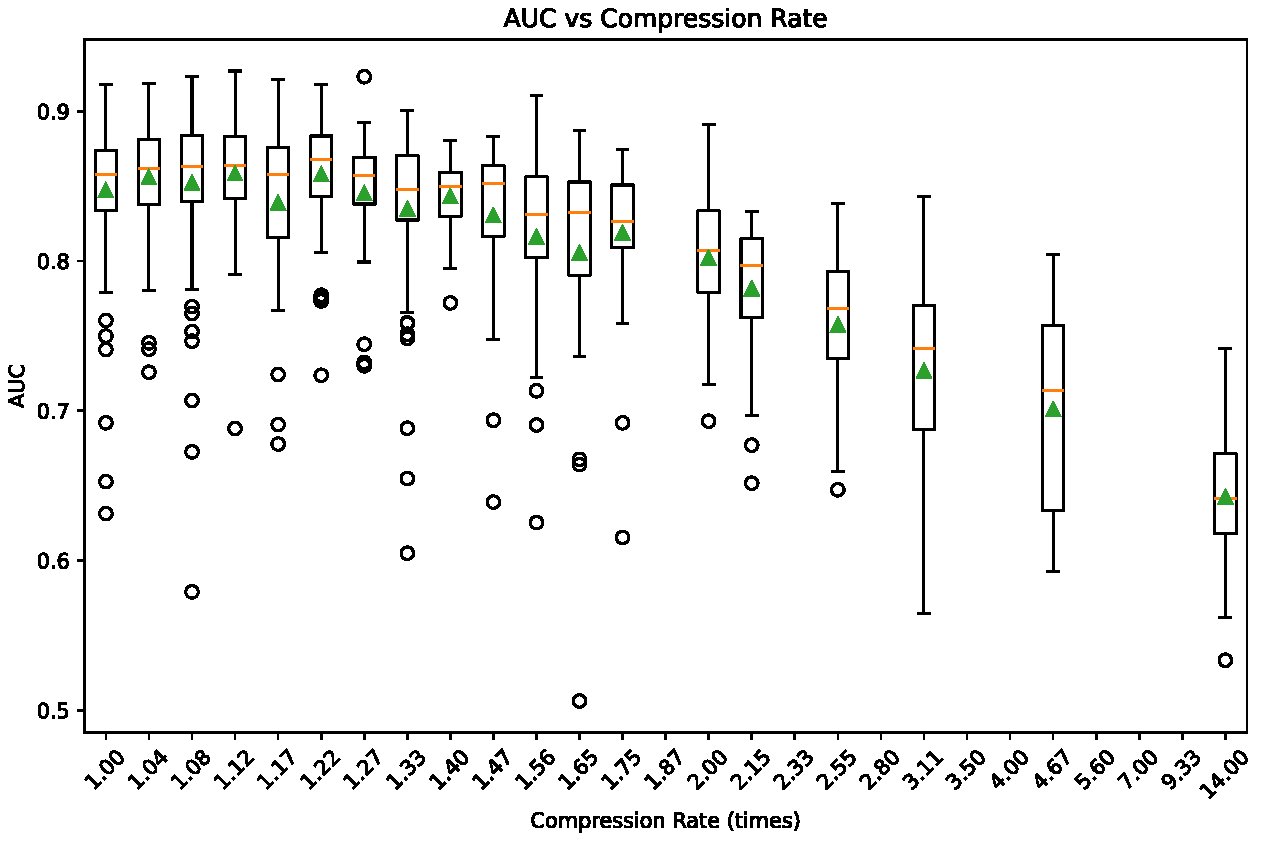
\includegraphics[width=1.2\textwidth]{search-compression-classify_model.pdf}



\section{Vanilla Autoencoder}
\label{sec:vanilla-ae}
For vanilla autoencoder, the concerns are mainly focused on the reconstruction quality of normal data and the ability to distinguish anomalies based on reconstruction errors.


\subsection{Reconstruction Quality on Normal Data}
To evaluate the reconstruction ability of the vanilla AE on normal operating conditions, we compute several standard metrics: mean average error (MAE), peak signal-to-noise ratio (PSNR), maximum reconstruction error, minimum reconstruction error, maximum min discrepancy and Wasserstein distance across time windows.

\begin{table}[h!]
\centering
\caption{Reconstruction metrics on normal validation data .}
\label{tab:rec_metrics_normal}
\begin{tabular}{lc}
\toprule
\textbf{Metric} & \textbf{Value} \\
\midrule
MAE                  & 0.0306 \\
PSNR [dB]            & 24.72 \\
Max error            & 0.1066 \\
Min error            & 0.0070 \\
Max--Min discrepancy & 0.0000 \\
Wasserstein distance & 0.0076 \\
\bottomrule
\end{tabular}
\end{table}

Overall, the reconstruction errors on normal validation data are low across all evaluated metrics, indicating that the vanilla AE learns to replicate healthy input signals with high fidelity. The mean absolute error (MAE) of $0.0306$ corresponds to a small deviation relative to the signal range, while the peak signal-to-noise ratio (PSNR) of $24.72$\,dB suggests a strong similarity between reconstructed and original signals. The maximum observed reconstruction error ($0.1066$) remains an order of magnitude smaller than typical anomaly-induced deviations, and the minimum error ($0.0070$) confirms that some time windows are reconstructed almost perfectly. The near-zero Max--Min discrepancy implies a consistent reconstruction quality across time windows, and the small Wasserstein distance ($0.0076$) shows that the overall error distribution closely matches that of the original data. These results confirm that the AE is capable of accurately modeling normal operating conditions.



\subsection{Normal vs. Abnormal Reconstruction}
For anomaly detection, the most straightforward approach is to use a static threshold on reconstruction error. For this study, ROC is first used to determine whether a significant difference exists in the reconstruction error between normal and abnormal samples.

\begin{table}[h!]
\centering
\caption{Feature-wise AUC for vanilla AE reconstruction error.}
\label{tab:vanilla_feat_auc}
\begin{tabular}{lc}
    \toprule
    \textbf{Feature} & \textbf{AUC} \\
    \midrule
    Power & 0.4449 \\
    Rotor speed & 0.5741 \\
    Wind speed & 0.4529 \\
    Air density & 0.6224 \\
    Temperature & 0.6163 \\
    Sin of Wind direction & 0.4499 \\
    Cos of Wind direction & 0.5460 \\
    \midrule
    \textbf{Overall} & \textbf{0.5036} \\
    \bottomrule
\end{tabular}
\end{table}

The overall AUC for the vanilla AE is close to 0.5, i.e., random performance, with feature-wise AUCs present in Table~\ref{tab:vanilla_feat_auc}.
The distribution of reconstruction errors for normal and abnormal validation samples is shown in Figure~\ref{fig:vanilla_norm_abnorm_roc}.

\begin{figure}[h!]
    \centering
    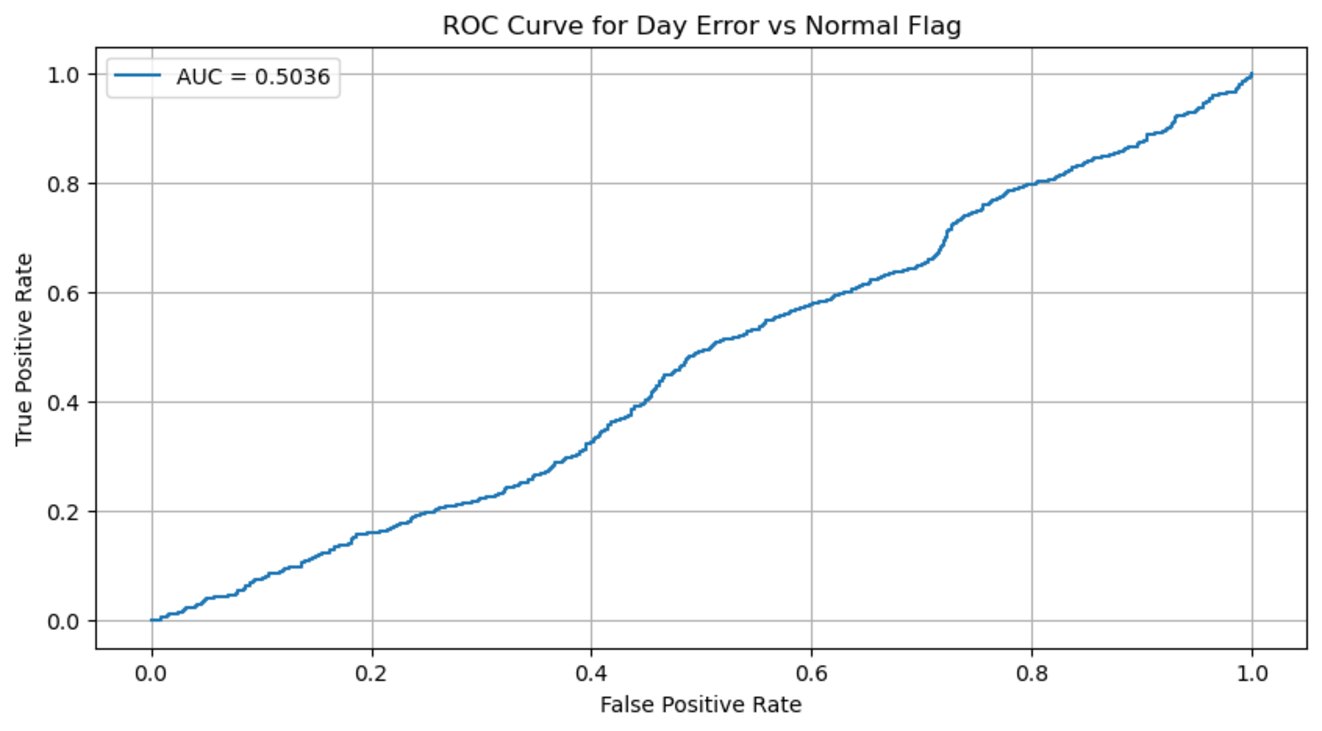
\includegraphics[width=\textwidth]{vanilla-roc.pdf}
    \caption{Vanilla AE ROC curve for normal vs. abnormal validation samples.}
    \label{fig:vanilla_norm_abnorm_roc}
\end{figure}


\begin{figure}[h!]
    \centering
    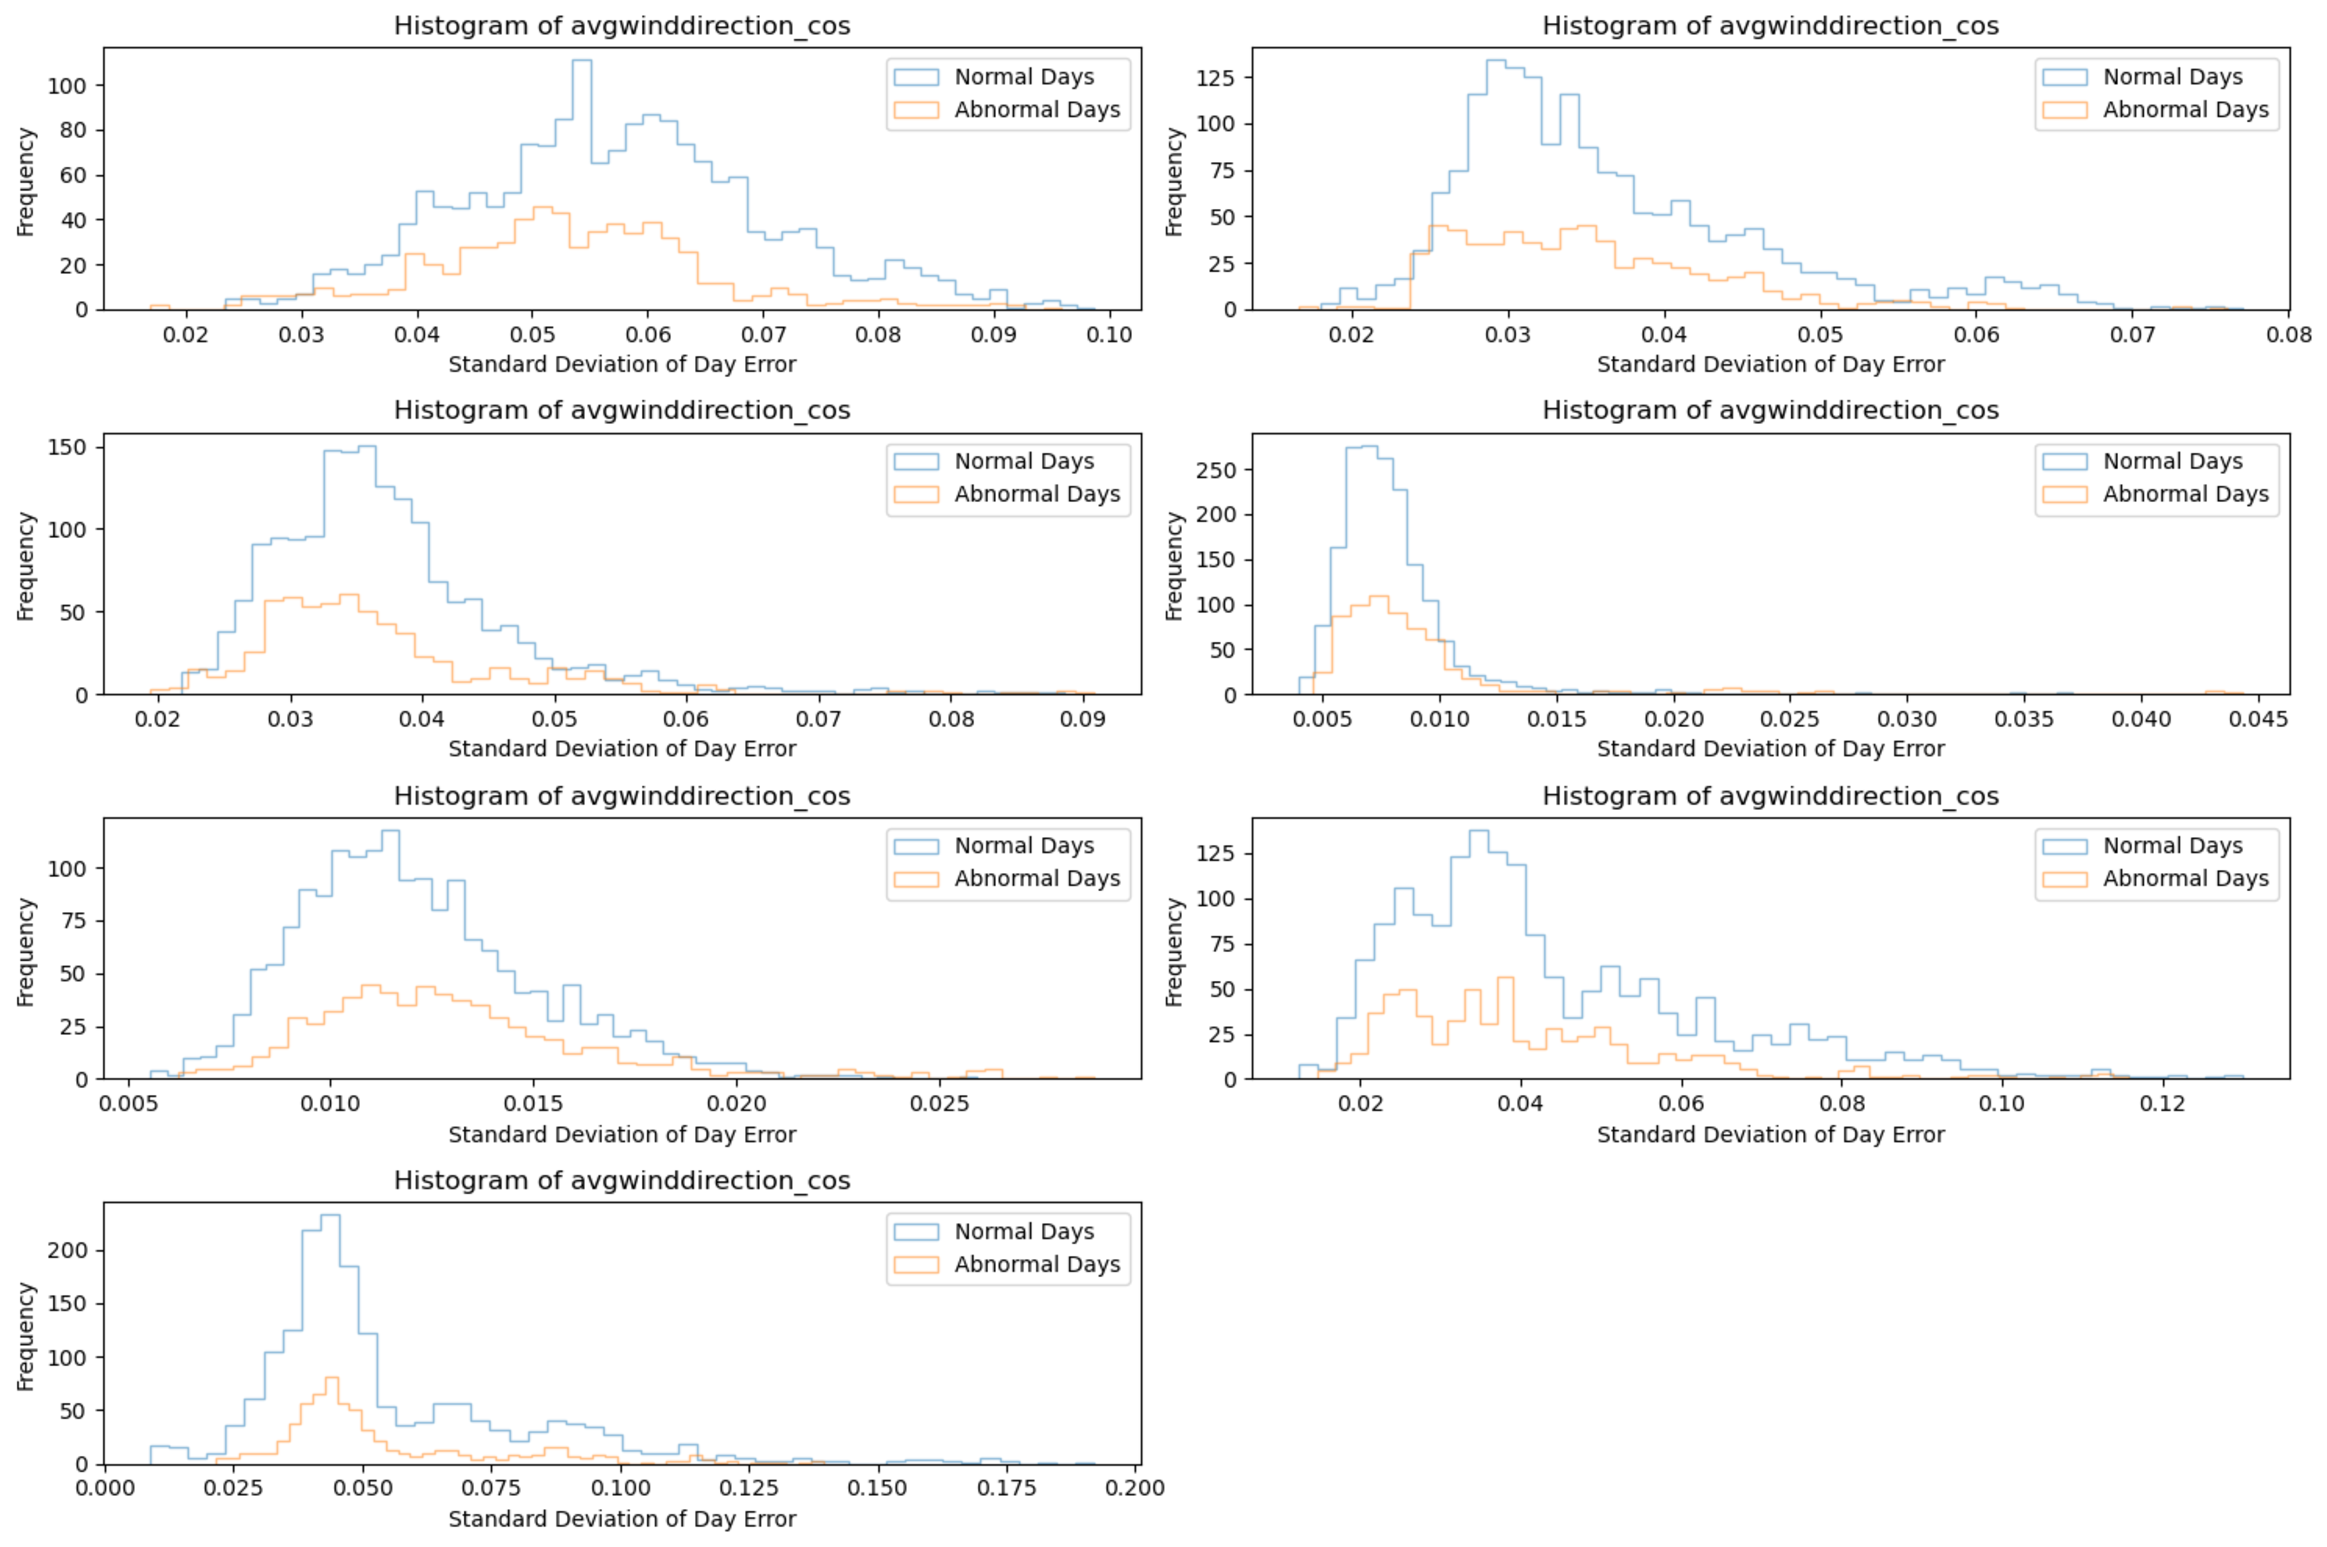
\includegraphics[width=\textwidth]{vanilla-reconst-hist.pdf}
    \caption{Vanilla AE reconstruction error (MSE) histogram for normal vs. abnormal validation samples.}
    \label{fig:vanilla_norm_abnorm_reconst_hist}
\end{figure}


Figure~\ref{fig:vanilla_norm_abnorm_reconst_hist}, Figure~\ref{fig:vanilla_norm_abnorm_roc} and Table~\ref{tab:vanilla_feat_auc} show that the vanilla AE is unable to create a linear separation between normal and abnormal samples based on reconstruction error. The AUC of $0.5036$ indicates that the model does not effectively distinguish between the two classes, as it is close to random guessing. The per-feature AUCs also suggest that some features provide a strong discrimination. It is easy to see that stable features such as air density and temperature have higher AUCs. These features are easier to reconstruct, thus, they are also more sensitive to anomalies.
However, they also did not provide enough information to achieve a meaningful separation overall.

\begin{figure}[h]
    \centering
    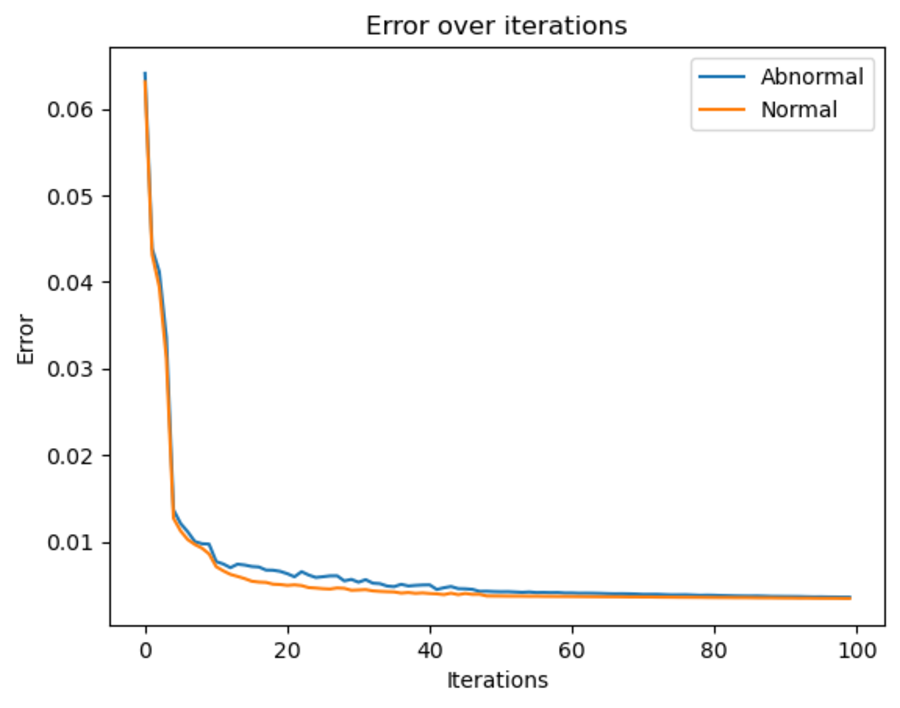
\includegraphics[width=0.85\textwidth]{vanilla-norm-abn-over-epoch.pdf}
    \caption{Reconstruction error (MSE) for normal and abnormal validation samples over training epochs.}
    \label{fig:vanilla_epoch_err}
\end{figure}

Given this poor separation, I further examined how reconstruction errors for normal and abnormal samples evolved throughout training (Figure~\ref{fig:vanilla_epoch_err}). Interestingly, the gap between the two classes is largest at around the 20th epoch, suggesting that the model initially learns to capture patterns specific to normal operating conditions while struggling to reconstruct abnormal signals. However, as training progresses, the reconstruction error for abnormal samples decreases to match that of normal samples. 
This convergence implies that the model gradually learns to represent both normal and abnormal patterns equally well, effectively "overfitting" to the anomalies present in the training set - the data that is nearly an abnormality. 
Consequently, the discriminative signal in reconstruction error is lost, explaining the near-random AUC observed in Table~\ref{tab:vanilla_feat_auc}.


This result suggests that either the difference in reconstruction error is highly non-linear and not captured by a simple threshold, or that the vanilla AE lacks the representational capacity for effective Normal Behavior Modeling in this dataset.




\subsection{Training Dynamics: Epoch-wise Behavior}
We monitor MSE over training epochs for both normal and abnormal validation sets.

\begin{figure}[h!]
    \centering
    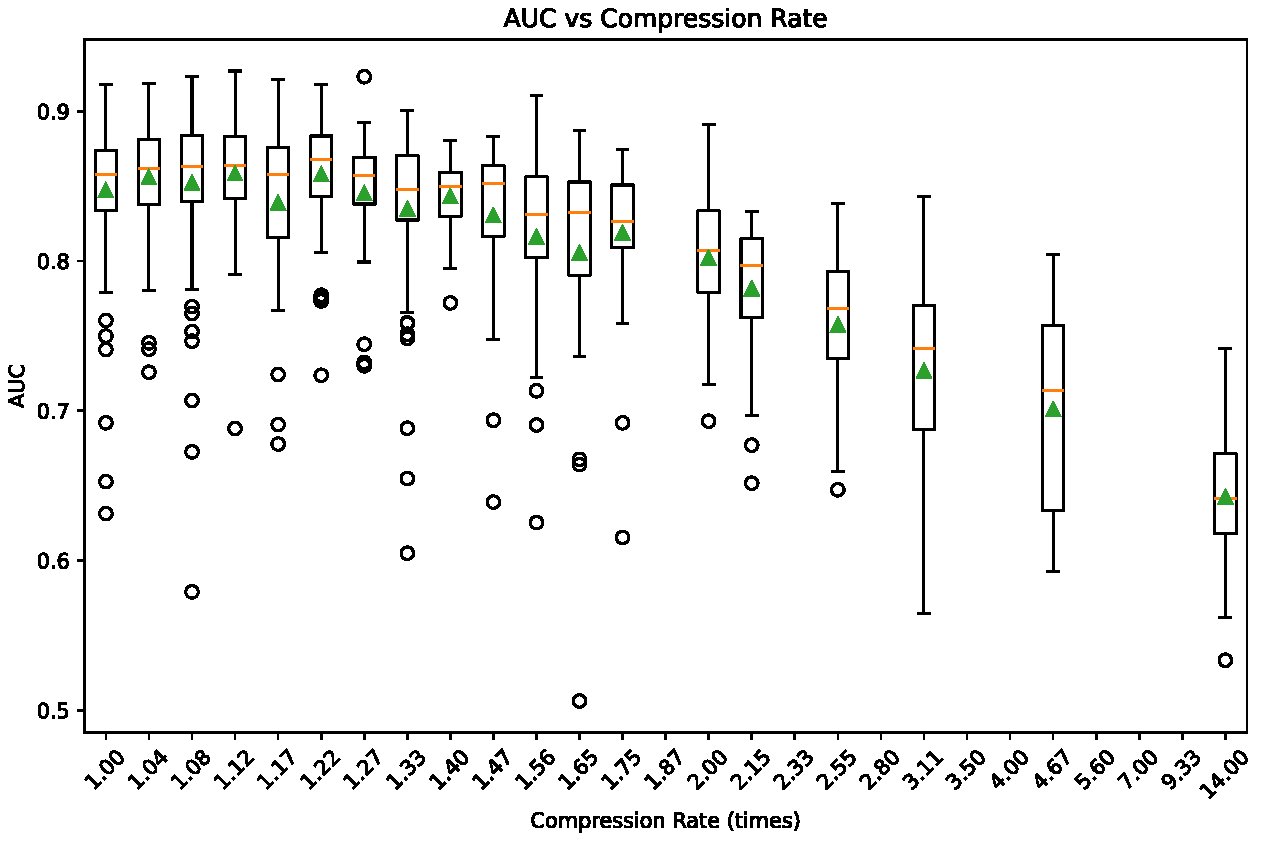
\includegraphics[width=0.85\textwidth]{search-compression-classify_model.pdf}
    \caption{Epoch-wise mean MSE for normal and abnormal validation sets. The difference $(\text{MSE}_{abn} - \text{MSE}_{norm})$ is also plotted.}
    \label{fig:vanilla_epoch_mse}
\end{figure}

As shown in Figure~\ref{fig:vanilla_epoch_mse}, \dots % interpretation

% ---------------------------------------------------------

\subsection{Aggregation Strategy Comparison}
Different aggregation strategies were applied to per-timestep errors for each window: mean, max, min, and $95^{\text{th}}$ percentile.

\begin{table}[h!]
\centering
\caption{Performance (AUC, F1, Precision, Recall) for different error aggregation strategies.}
\label{tab:agg_strategies}
\begin{tabular}{lcccc}
\toprule
\textbf{Aggregator} & \textbf{AUC} & \textbf{F1} & \textbf{Precision} & \textbf{Recall} \\
\midrule
Mean       & <value> & <value> & <value> & <value> \\
Max        & <value> & <value> & <value> & <value> \\
Min        & <value> & <value> & <value> & <value> \\
P95        & <value> & <value> & <value> & <value> \\
\bottomrule
\end{tabular}
\end{table}

\begin{figure}[h!]
    \centering
    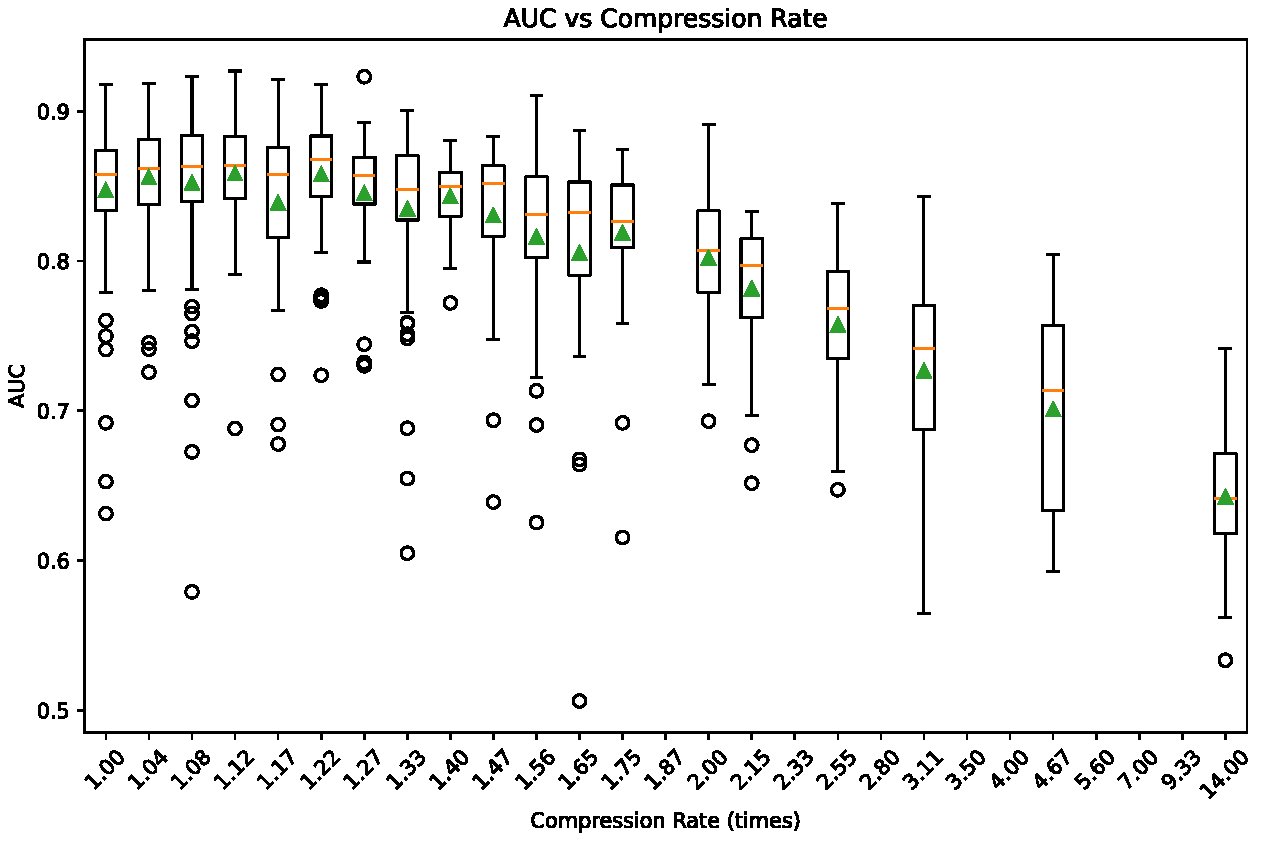
\includegraphics[width=0.85\textwidth]{search-compression-classify_model.pdf}
    \caption{ROC curves for different error aggregation strategies.}
    \label{fig:vanilla_roc_aggregators}
\end{figure}

% ---------------------------------------------------------

\subsection{Latent Size Sweep}
We evaluate the effect of latent size on reconstruction and detection performance.

\begin{table}[h!]
\centering
\caption{Effect of latent size on reconstruction and anomaly separability.}
\label{tab:latent_sweep}
\begin{tabular}{cccc}
\toprule
\textbf{Latent size} & \textbf{MSE$_{norm}$} & \textbf{MSE$_{abn}$} & \textbf{AUC} \\
\midrule
2   & <value> & <value> & <value> \\
4   & <value> & <value> & <value> \\
8   & <value> & <value> & <value> \\
16  & <value> & <value> & <value> \\
32  & <value> & <value> & <value> \\
64  & <value> & <value> & <value> \\
\bottomrule
\end{tabular}
\end{table}

\begin{figure}[h!]
    \centering
    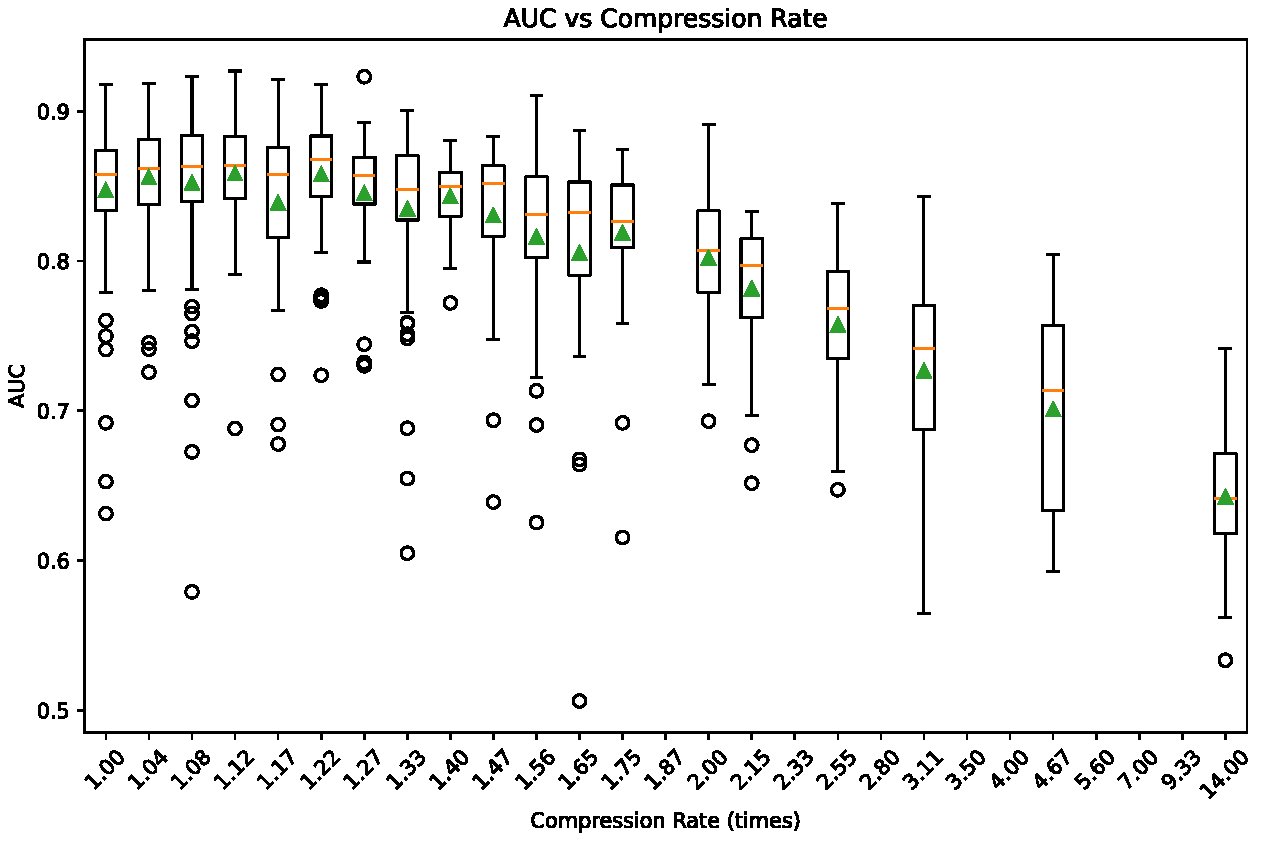
\includegraphics[width=0.85\textwidth]{search-compression-classify_model.pdf}
    \caption{AUC vs latent size.}
    \label{fig:vanilla_latent_auc}
\end{figure}

% ---------------------------------------------------------

\subsection{Per-feature Error Analysis}
Per-feature MSE was computed for normal and abnormal sets to identify which sensors contributed most to anomaly separability.

\begin{figure}[h!]
    \centering
    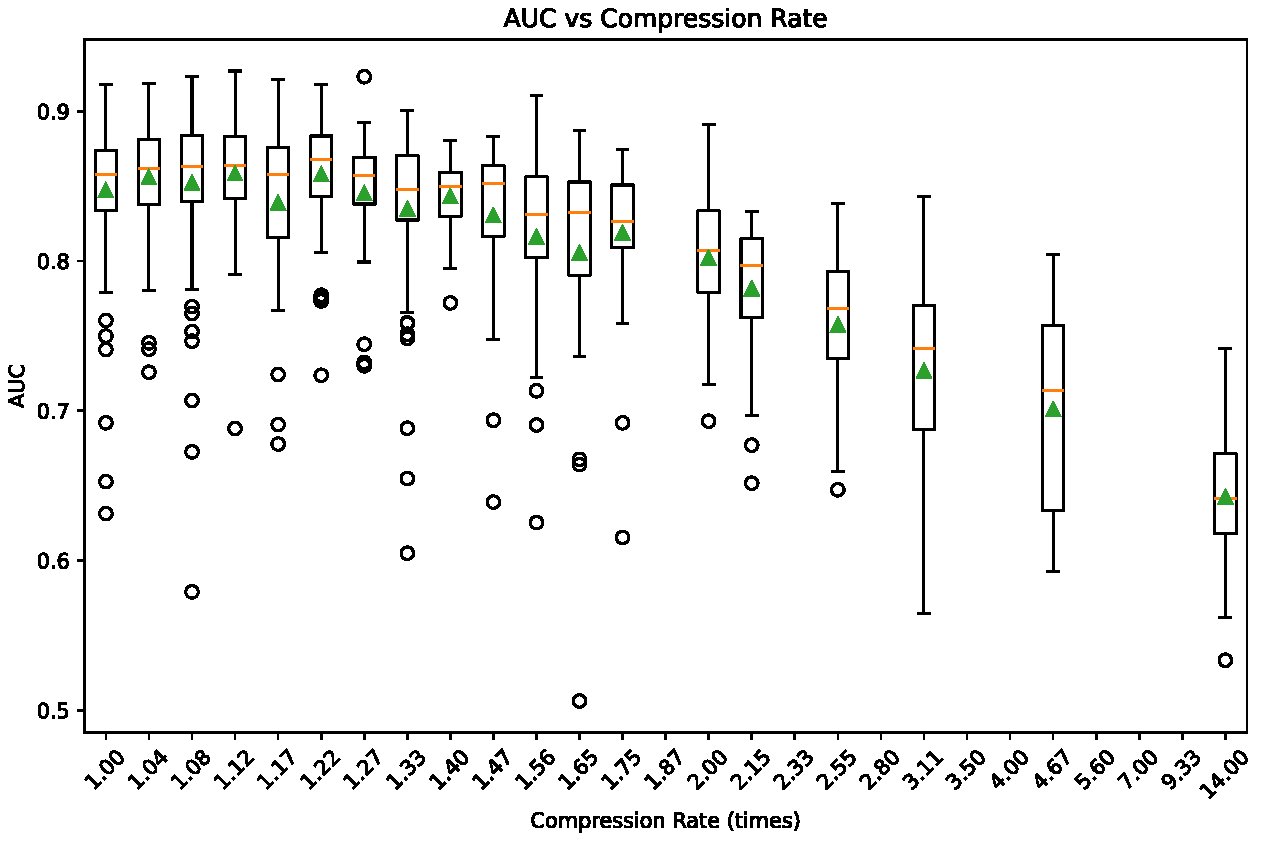
\includegraphics[width=0.9\textwidth]{search-compression-classify_model.pdf}
    \caption{Heatmap of per-feature MSE for normal and abnormal samples.}
    \label{fig:vanilla_feature_error_heatmap}
\end{figure}

\subsection{Summary}
In summary, the vanilla AE \dots % Your conclusion here.

% ------------------- chapter -------------------
%This is the extract from ICSBT article.
\chapter{Conclusions}



% ------------------- paths to graphics -------------------

% change according to folder and file names
\ifpdf
    \graphicspath{{6_conclusions/figures/}{6_conclusions/figures/}
            {6_conclusions/figures/}}
\else
    \graphicspath{{6_conclusions/figures/EPS/}{6_conclusions/figures/}}
\fi


% --------------------------------------------------------------
%:                  BACK MATTER: appendices, refs,..
% --------------------------------------------------------------

% the back matter: appendix and references close the thesis

\color{black}

% here we start the Appendix
\appendix

% Definition of each Chapter in the Appendix is done via the following two lines
\chapter*{Appendix A}


\addcontentsline{toc}{chapter}{Appendix A: Dataset Details}
\chaptermark{Appendix}
\markboth{Appendix}{Appendix}
% here is how we close the chapter




%: ----------------------- bibliography ------------------------
    

\begin{small}
\bibliographystyle{plainnat}
\renewcommand{\bibname}{References}
% {References} 
\bibliography{references} 
\end{small}

% -------------------------------------------------------------

\end{document}
